\chapter{Glauber modeling}\label{chap:glauber}

\section{$\avgNcoll$ for minimum bias collisions}\label{sec:ncoll_glauber}
The present $\RAA$ measurement is performed without centrality differentiation, i.e., integrated over the available impact parameter $b$ range. Calculation of $\avgNcoll$ is performed in the Monte-Carlo Glauber (MCG) approach using publicly available code of TGlauberMC \cite{alver2008phobosglaubermontecarlo, PhysRevC.97.054910}.

There are several input parameters to TGlauberMC:
\begin{enumerate}
    \item Inelastic nucleon-nucleon cross-section $\sigma_{_\mathrm{NN}}$. For $\sqn = \qty{5.36}{\tev}$ it is taken as $\sigma_{_\mathrm{NN}}= \sigma_{\pp} =~68.2\pm~\qty{0.6}{mb}$ from \cite{PhysRevC.97.054910} as linear interpolation between 5.02 and 5.44 TeV
    \item Minimal distance between nucleons $d_\text{min}$ with a default value of $d_\text{min} = \qty{0.4}{fm}$ %In the improved version, a space lattice is introduced with separation $d_\text{node}$
    \item Geometric model of colliding nuclei. Three models for oxygen are available (in TGlauberMC): harmonic-oscillator model, Woods-Saxon parametrization (3-parameter Fermi, 3pF), and a model based on direct wave-function calculation. For neon 3pF parametrization was implemented with parameters taken from \cite{DEVRIES1987495}
    % \item Nucleon collision profile
    % \begin{equation}
    %     P(b_{NN}) = \Gamma \left(1/\omega, b_{NN}/D^2\omega \right) / \Gamma (1/\omega)
    % \end{equation}
    % with parameter $\omega$, with $\omega=0$ reducing to "black-disk" approximation, and with $\omega=1$ to Gaussian profile. Value of $\omega=0.4$ is quoted to reproduce $\pp$ cross-sections at LHC energies \cite{PhysRevC.97.054910}, and therefore is taken as default
    % \item Event-by-event fluctuations of $\sigma_{NN}$ (color fluctuations inside nucleons):
    % \begin{equation}
    %     P_\sigma(\sigma_{NN}) = C \frac{\sigma_{NN}}{\sigma_{NN} + \sigma_0}\exp{\left(-\left[\frac{\sigma_{NN}-\sigma_0}{\sigma_0\Omega}\right]^2\right)}
    % \end{equation}
\end{enumerate}

Resulting distributions of $\Ncoll$ and $\Npart$ for $\OO$ calculated in TGlauberMC (with two different geometry models) and for $\NeNe$ are presented in Figure~\ref{fig:ncoll_npart_oo}
\begin{figure}[h]
    \centering
    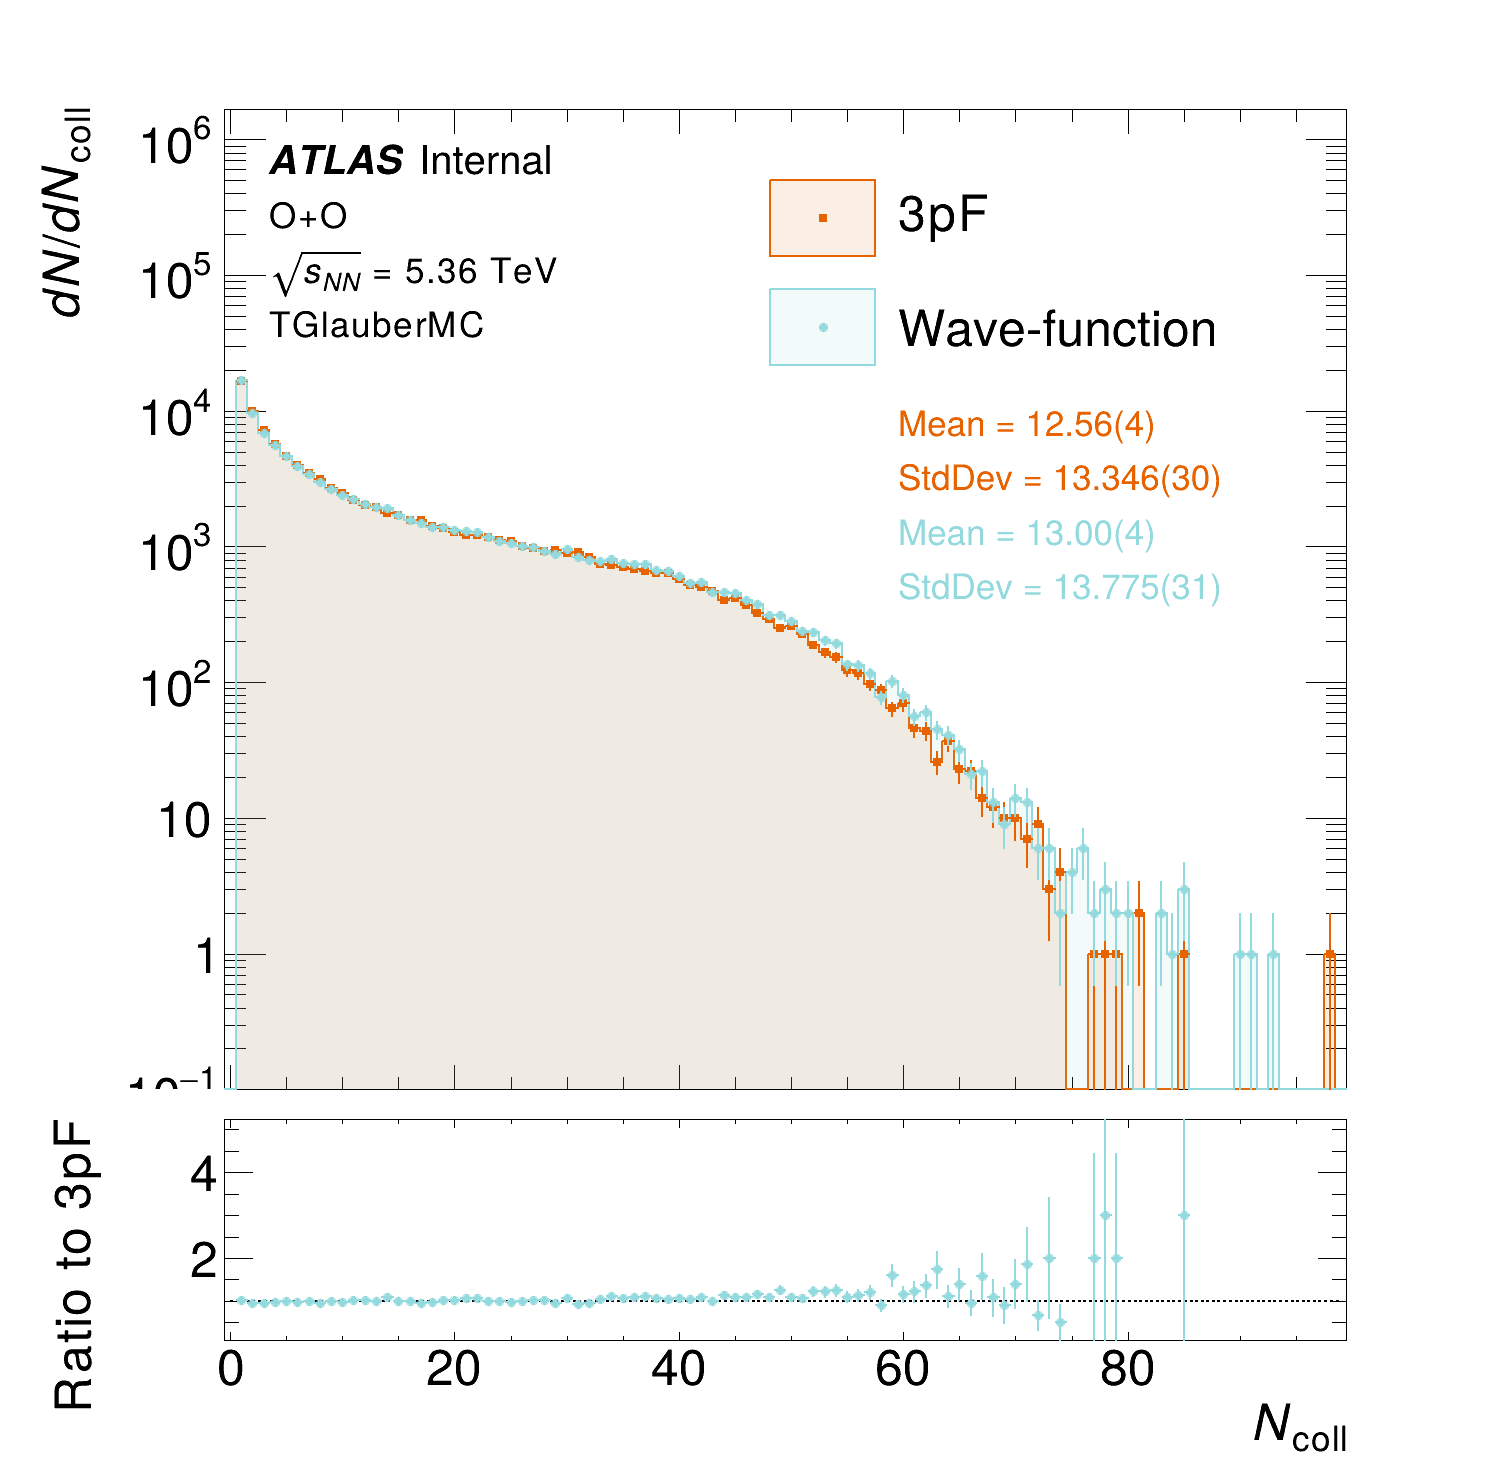
\includegraphics[width=0.49\linewidth]{images/NcollOO.png}
    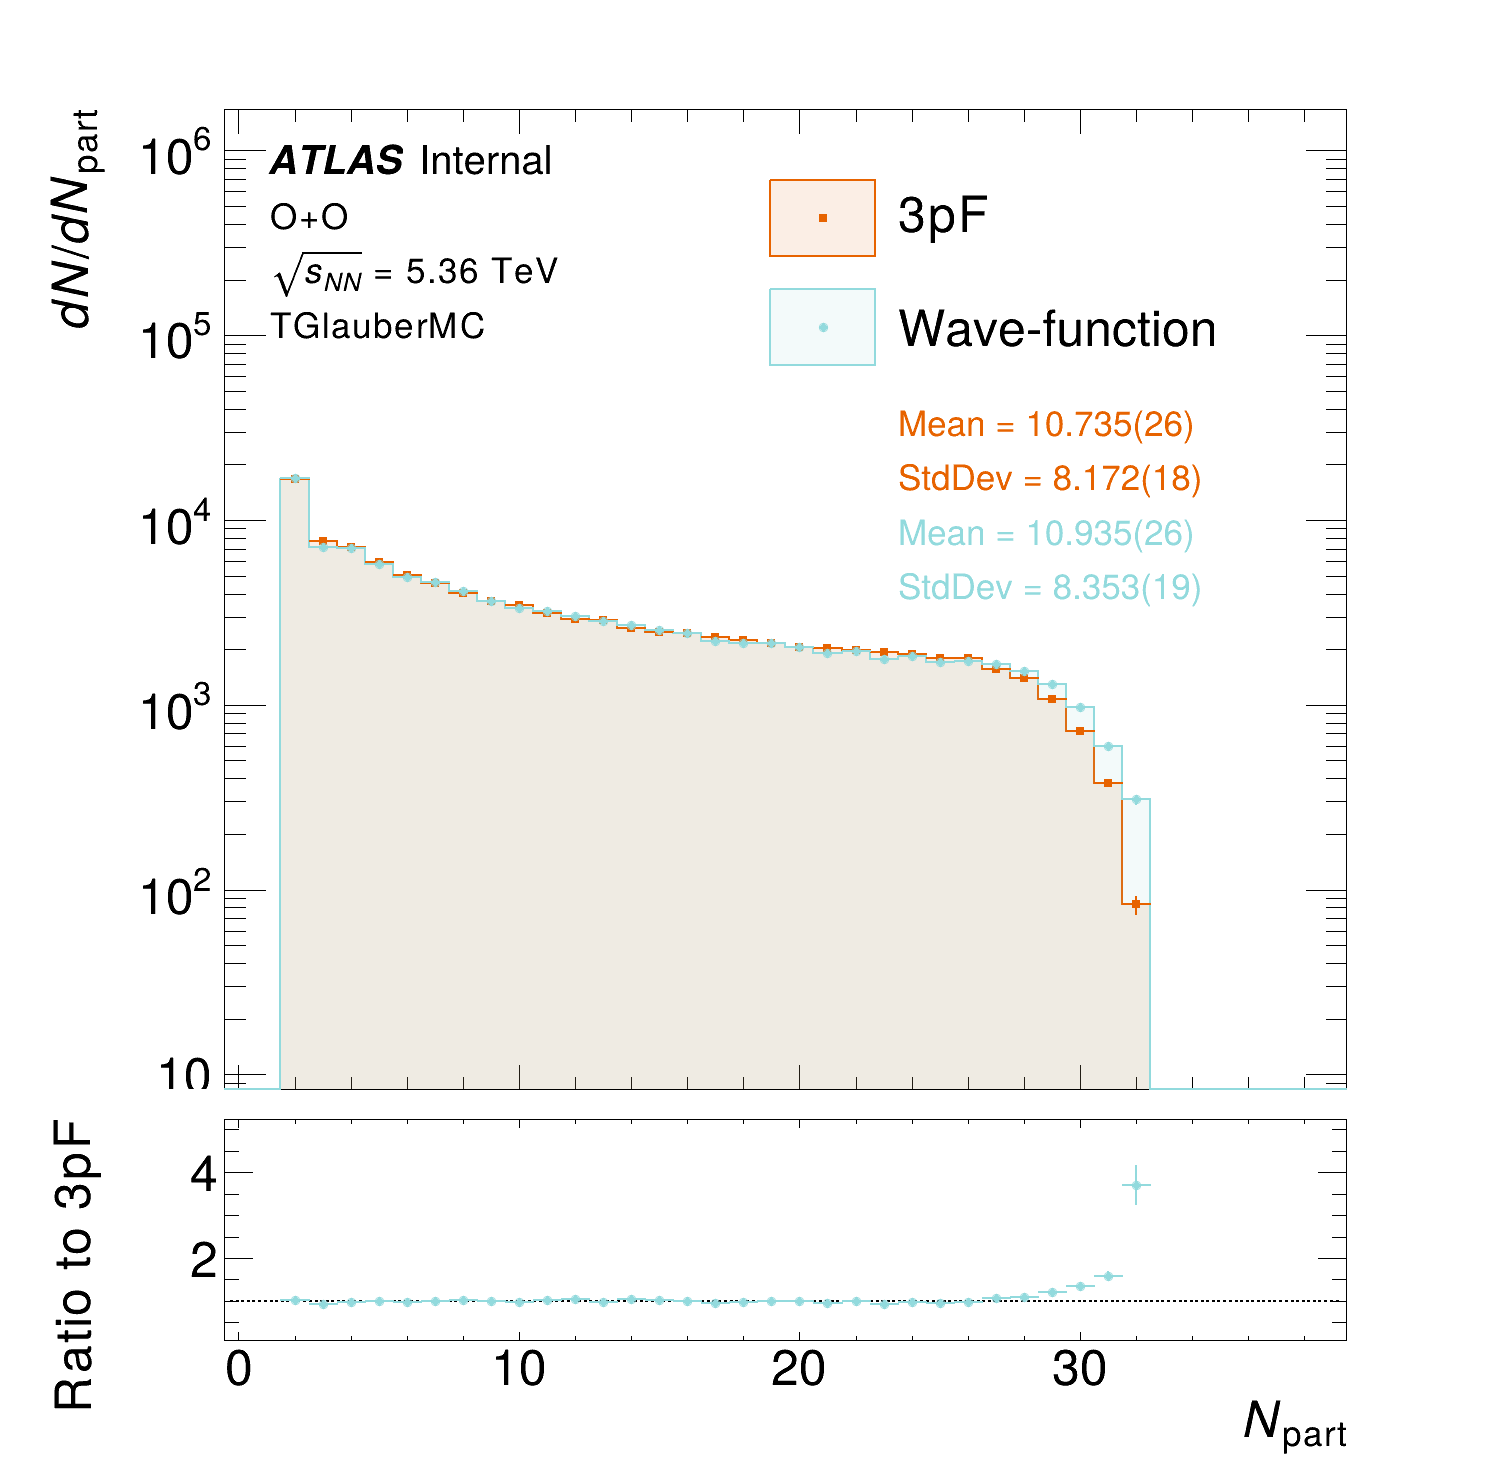
\includegraphics[width=0.49\linewidth]{images/NpartOO.png}
    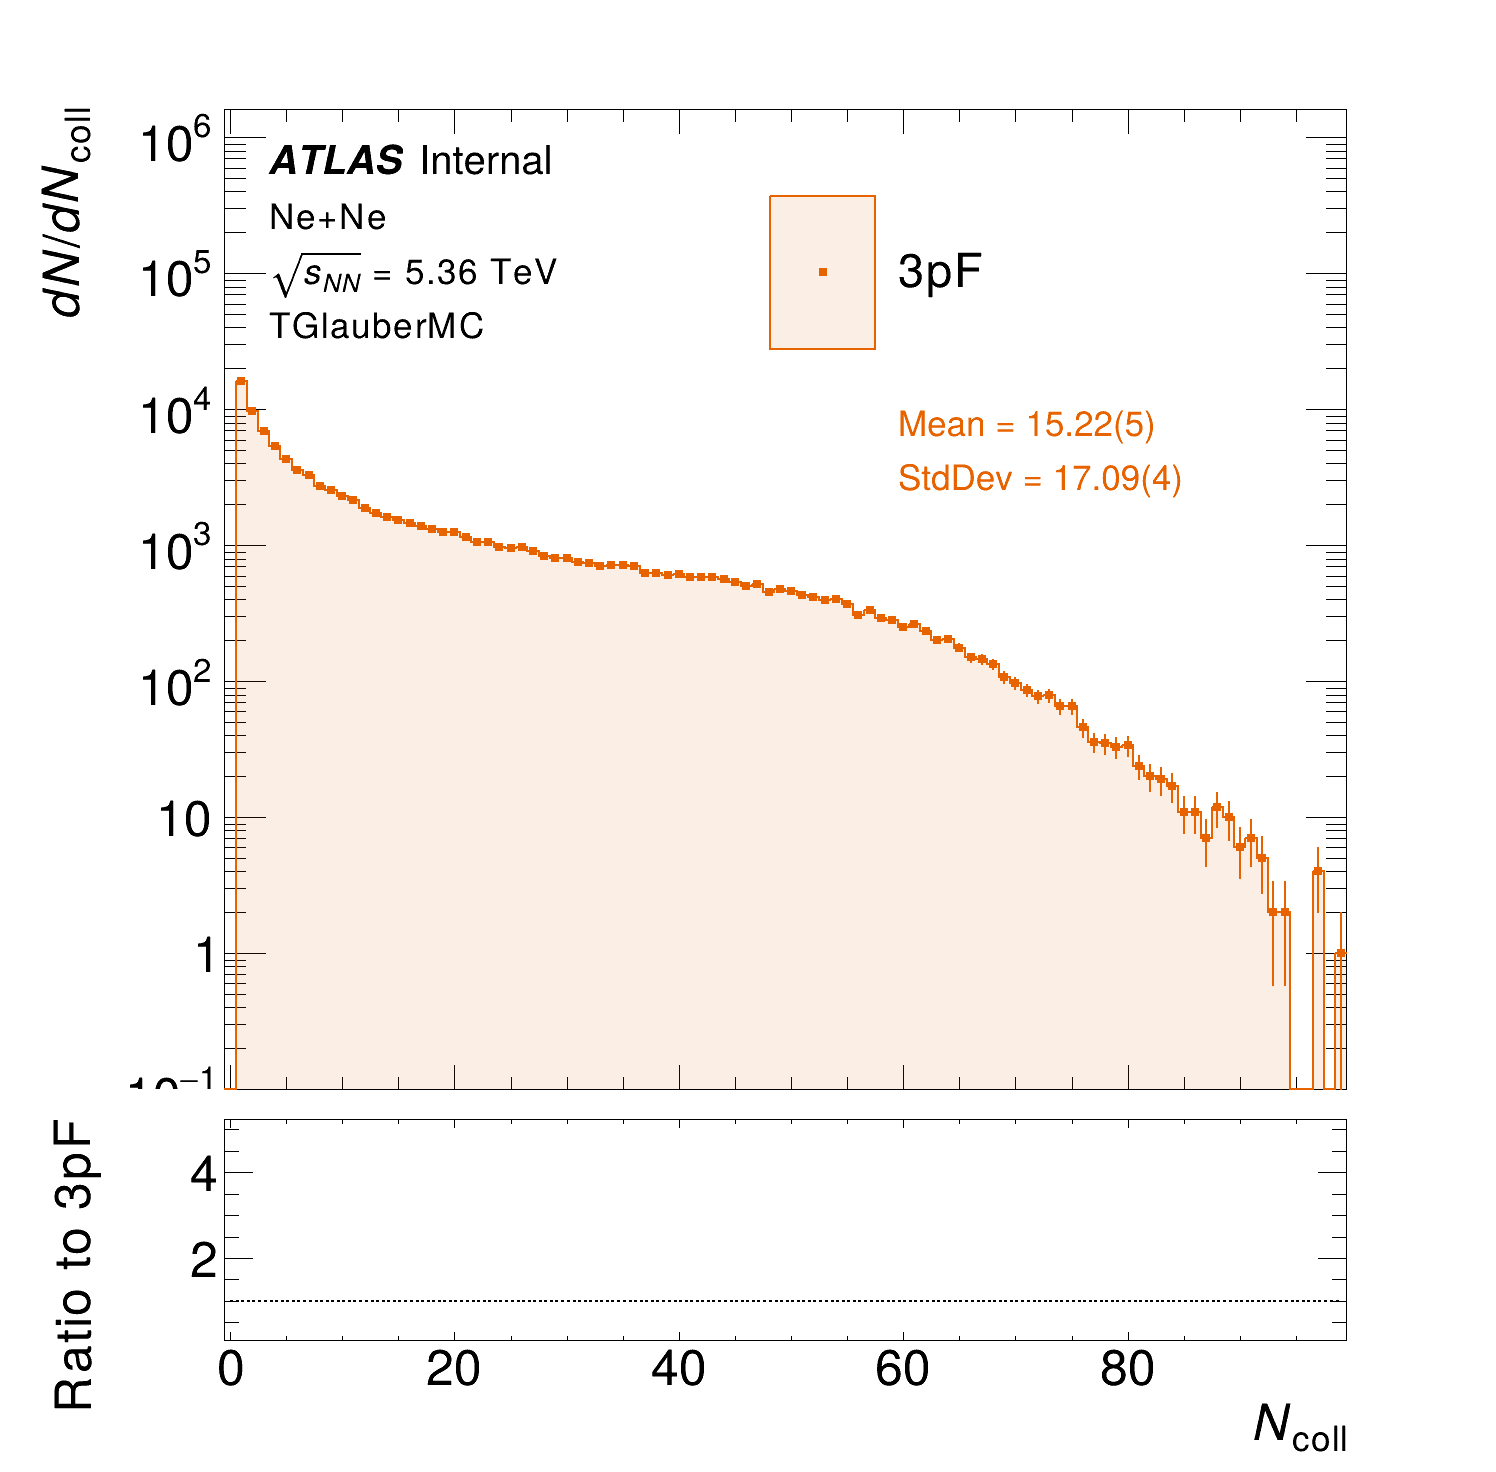
\includegraphics[width=0.49\linewidth]{images/NcollNeNe.png}
    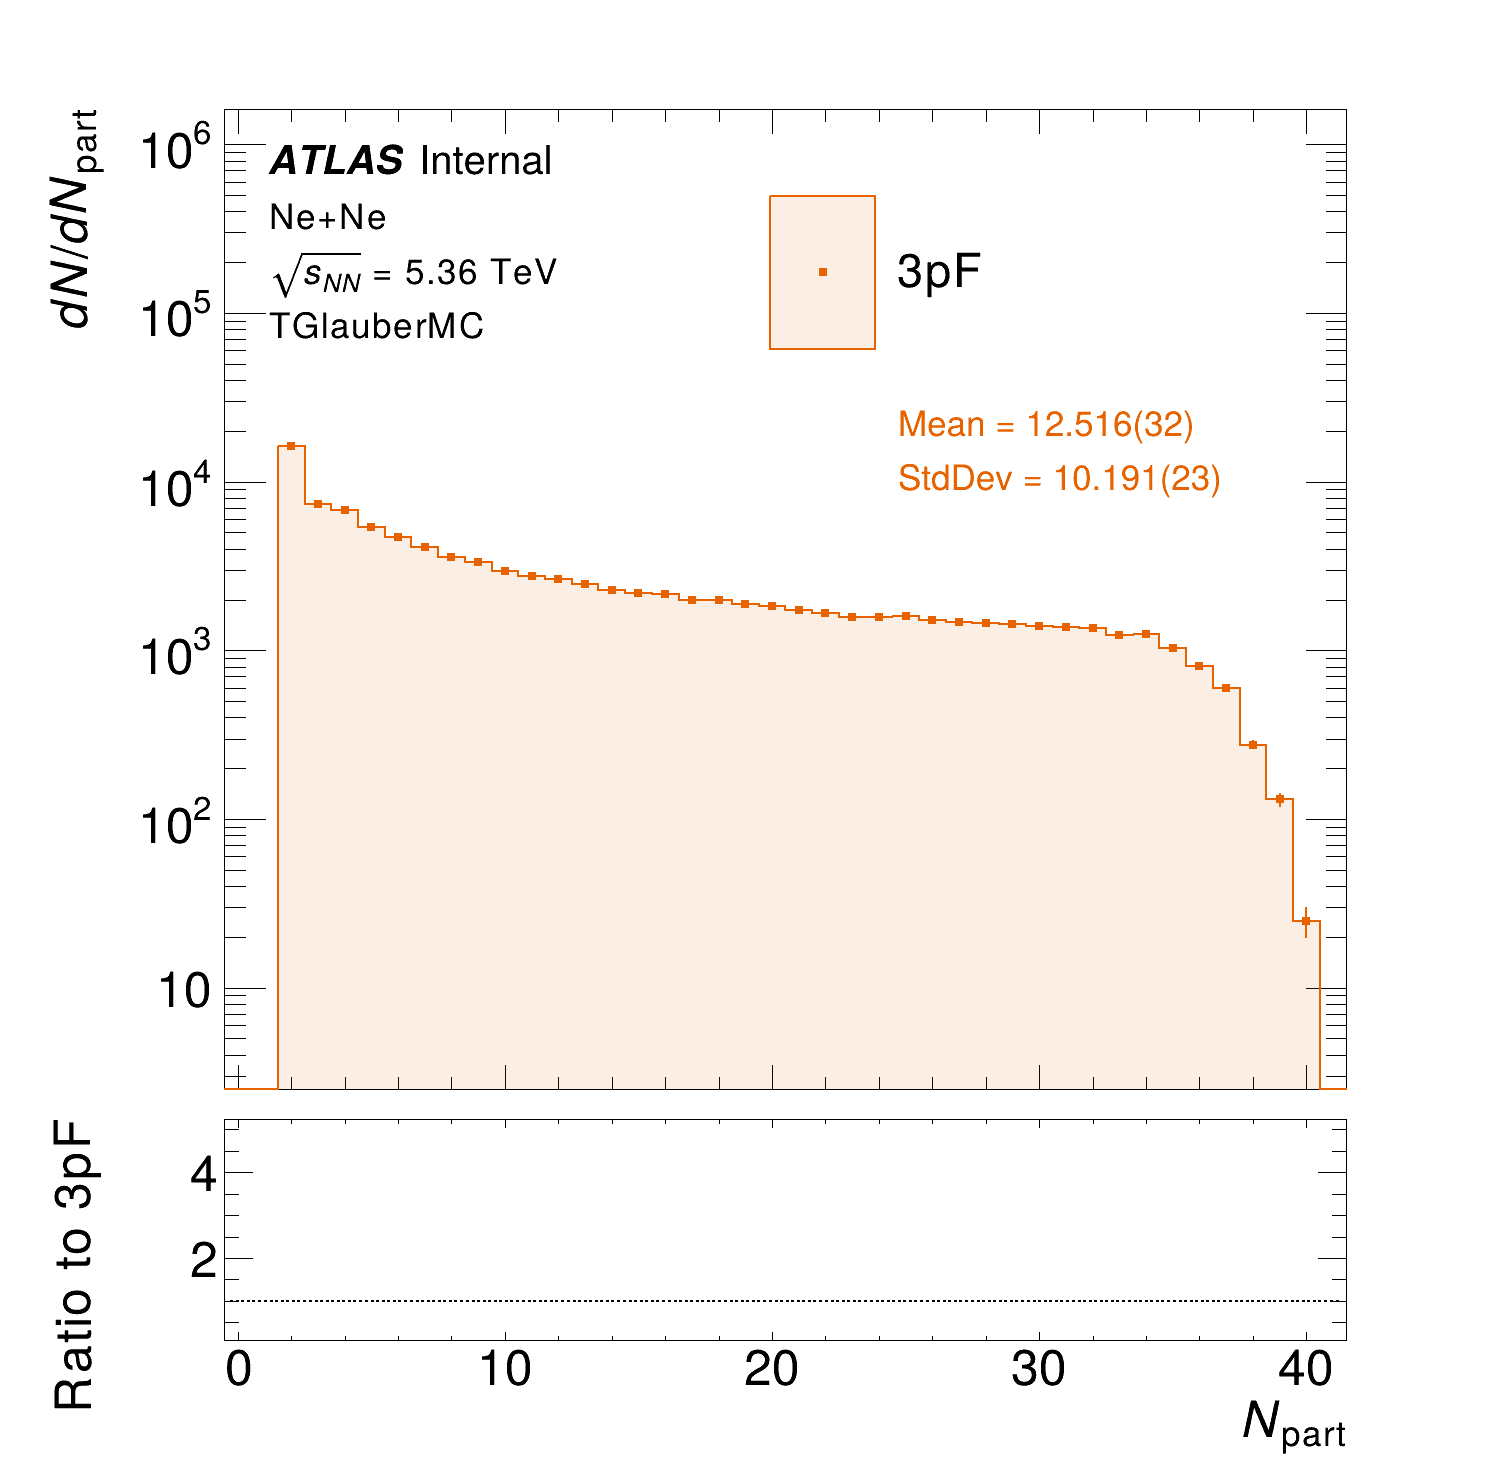
\includegraphics[width=0.49\linewidth]{images/NpartNeNe.png}
    \caption{Top: distributions of $\Ncoll$ and $\Npart$ in $\OO$. Bottom: distributions of $\Ncoll$ and $\Npart$ in $\NeNe$}
    \label{fig:ncoll_npart_oo}
\end{figure}
